

\documentclass[]{report}

\voffset=-1.5cm
\oddsidemargin=0.0cm
\textwidth = 480pt

\usepackage{framed}
\usepackage{subfiles}
\usepackage{graphics}
\usepackage{newlfont}
\usepackage{eurosym}
\usepackage{amsmath,amsthm,amsfonts}
\usepackage{amsmath}
\usepackage{enumerate}
\usepackage{color}
\usepackage{multicol}
\usepackage{amssymb}
\usepackage{multicol}
\usepackage[dvipsnames]{xcolor}
\usepackage{graphicx}
\begin{document}
\section*{Question 30 - Backward Induction}
The service provider, player I, makes the first move, choosing High or Low quality of
service. Then the customer, player II, is informed about that choice. Player II can then
decide separately between buy and don’t buy in each case. 
The resulting payoffs are depicted on the tree.
	\begin{figure}[h!]
\centering
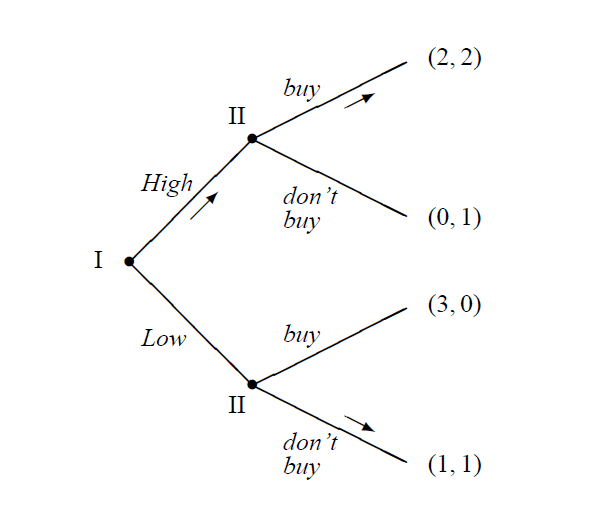
\includegraphics[width=0.45\linewidth]{C:/Users/kevin.obrien/Documents/GitHub/OperationsResearch2/Ramsey/Q30}

\end{figure}

\subsection*{Solution}
\begin{itemize}
\item This technique solves the game by first considering the last possible choices in the game.
Here, player II moves last. Since she knows the play will end after her move, she can
safely select the action which is best for her. 
\begin{itemize}
\item If player I has chosen to provide high quality
service, then the customer prefers to buy, since her resulting payoff of 2 is larger
than 1 when not buying. 
\item If the provider has chosen Low, then the customer prefers not to
purchase.
\end{itemize}
 
\item These choices by player II are indicated by arrows.
Once the last moves have been decided, backward induction proceeds to the players
making the next-to-last moves (and then continues in this manner). 
\item Player I
makes the next-to-last move, which in this case is the first move in the game. Being
rational, he anticipates the subsequent choices by the customer. 
\item He therefore realizes
that his decision between High and Low is effectively between the outcomes with payoffs
(2; 2) or (1; 1) for the two players, respectively.
\item  Clearly, he prefers High, which results in
a payoff of 2 for him, to Low, which leads to an outcome with payoff 1.
\item \textbf{OUTCOME} So the unique
solution to the game, as determined by backward induction, is that player I offers highquality
service, and player II responds by buying the service.
\end{itemize}

\end{document}